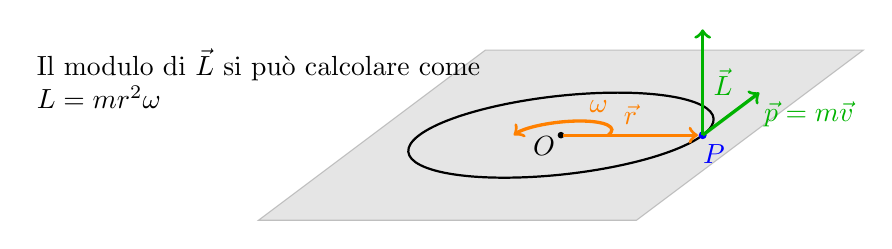
\begin{tikzpicture}[scale=1.2, x={(1cm,0cm)}, y={(0.4cm,0.3cm)}, z={(0cm,0.7cm)}]

    % Piano grigio con ombra
    \fill[gray!20] (-2,-3,0) -- (2,-3,0) -- (2,3,0) -- (-2,3,0) -- cycle;
    \draw[gray!50] (-2,-3,0) -- (2,-3,0) -- (2,3,0) -- (-2,3,0) -- cycle;

    % Cerchio sul piano (leggermente inclinato)
    \draw[thick] (0,0,0) circle (1.5);

    % Punto O
    \fill (0,0,0) circle (1.0pt);
    \node[left] at (0.2,-0.4,0) {$O$};

    % Punto P
    \fill[blue] (1.5,0,0) circle (1.2pt);
    \node[blue, below right] at (1.4,0,0) {$P$};

    % Vettore r
    \draw[->,very thick, orange] (0.02,0,0) -- (1.45,0,0) node[midway, above] {$\vec{r}$};

    % Vettore omega (curvo)
    \draw[->, very thick, orange] (0.5,0,0) arc (0:180:0.5);
    \node[orange] at (0,1,0) {$\omega$};

    % Vettore p = m v
    \draw[->, very thick, green!70!black] (1.5,0,0) -- (1.5,1.5,0) node[midway, right=8pt] {$\vec{p}=m\vec{v}$};

    % Vettore L (più lungo e ben visibile)
    \draw[->, very thick, green!70!black] (1.5,0,0) -- (1.5,0,1.6) node[midway, right] {$\vec{L}$};

    % Testo esplicativo (spostato fuori dal piano)
    \node[align=left] at (-4,2,0) {Il modulo di $\vec{L}$ si può calcolare come\\
    $L = m r^2 \omega$};

\end{tikzpicture}

